\chapter{Geladenes Teilchen im elektrischen Feld\label{chapter:efeld}}
\lhead{Teilchen im elektrischen Feld}
\begin{refsection}
\chapterauthor{Michael Cerny und Stefan Schindler}


In diesem Kapitel erweitern wir das Beispiel des Potentialkastens 
(Kapitel \ref{subsection:potentialkasten}, Seite \pageref{subsection:potentialkasten})
um eine St\"orung.

\section{Grundlagen St"orungstheorie}
Grunds"atzlich k"onnen wir mit der St\"orungstheorie ein einfaches Modell 
(Abb \ref{abb:efeld_psi_ungestoert} der ersten 5 Energieniveaus) 
mit einer St\"orung erg"anzen, statt von Anfang an mit einem komplexen Modell zu rechnen.

Allgemein gilt:
\[
  f(x, \varepsilon) = f_0(x) + \varepsilon f_1(x) + \varepsilon^2 f_2(x) + \ldots + \varepsilon^n f_n(x)
\]
Dabei ist $f_0(x)$ die urspr\"ungliche Funktion und $f_n(x)$ die $n$-te  N"aherung der St"orung.
Mit $\varepsilon$ wird die St"orung gesteuert. Dabei sollte $\varepsilon$ nicht zu gross gew"ahlt werden, 
da die N"aherung sonst ungenau wird. 

Setzen wir $\varepsilon = 0$, k\"onnen wir die St"orung dynamisch abschalten.

In der Quantenmechanik k"onnen wir die St"orungstheorie anwenden indem wir den Hamilton-Operator der 
urspr"unglichen Funktion $H_0$ um zus"atzliche $\varepsilon^n H_n$ erg"anzen:
\[
  H = \varepsilon^0 H_0 + \varepsilon^1 H_1 + \varepsilon^2 H_2 + \ldots + \varepsilon^n \hat H_n
\]












\section{Anwendungen}

\subsection{Potentialkasten mit elektrischem Feld}

\subsubsection{Ausgangslage}

\begin{figure}
 \centering
 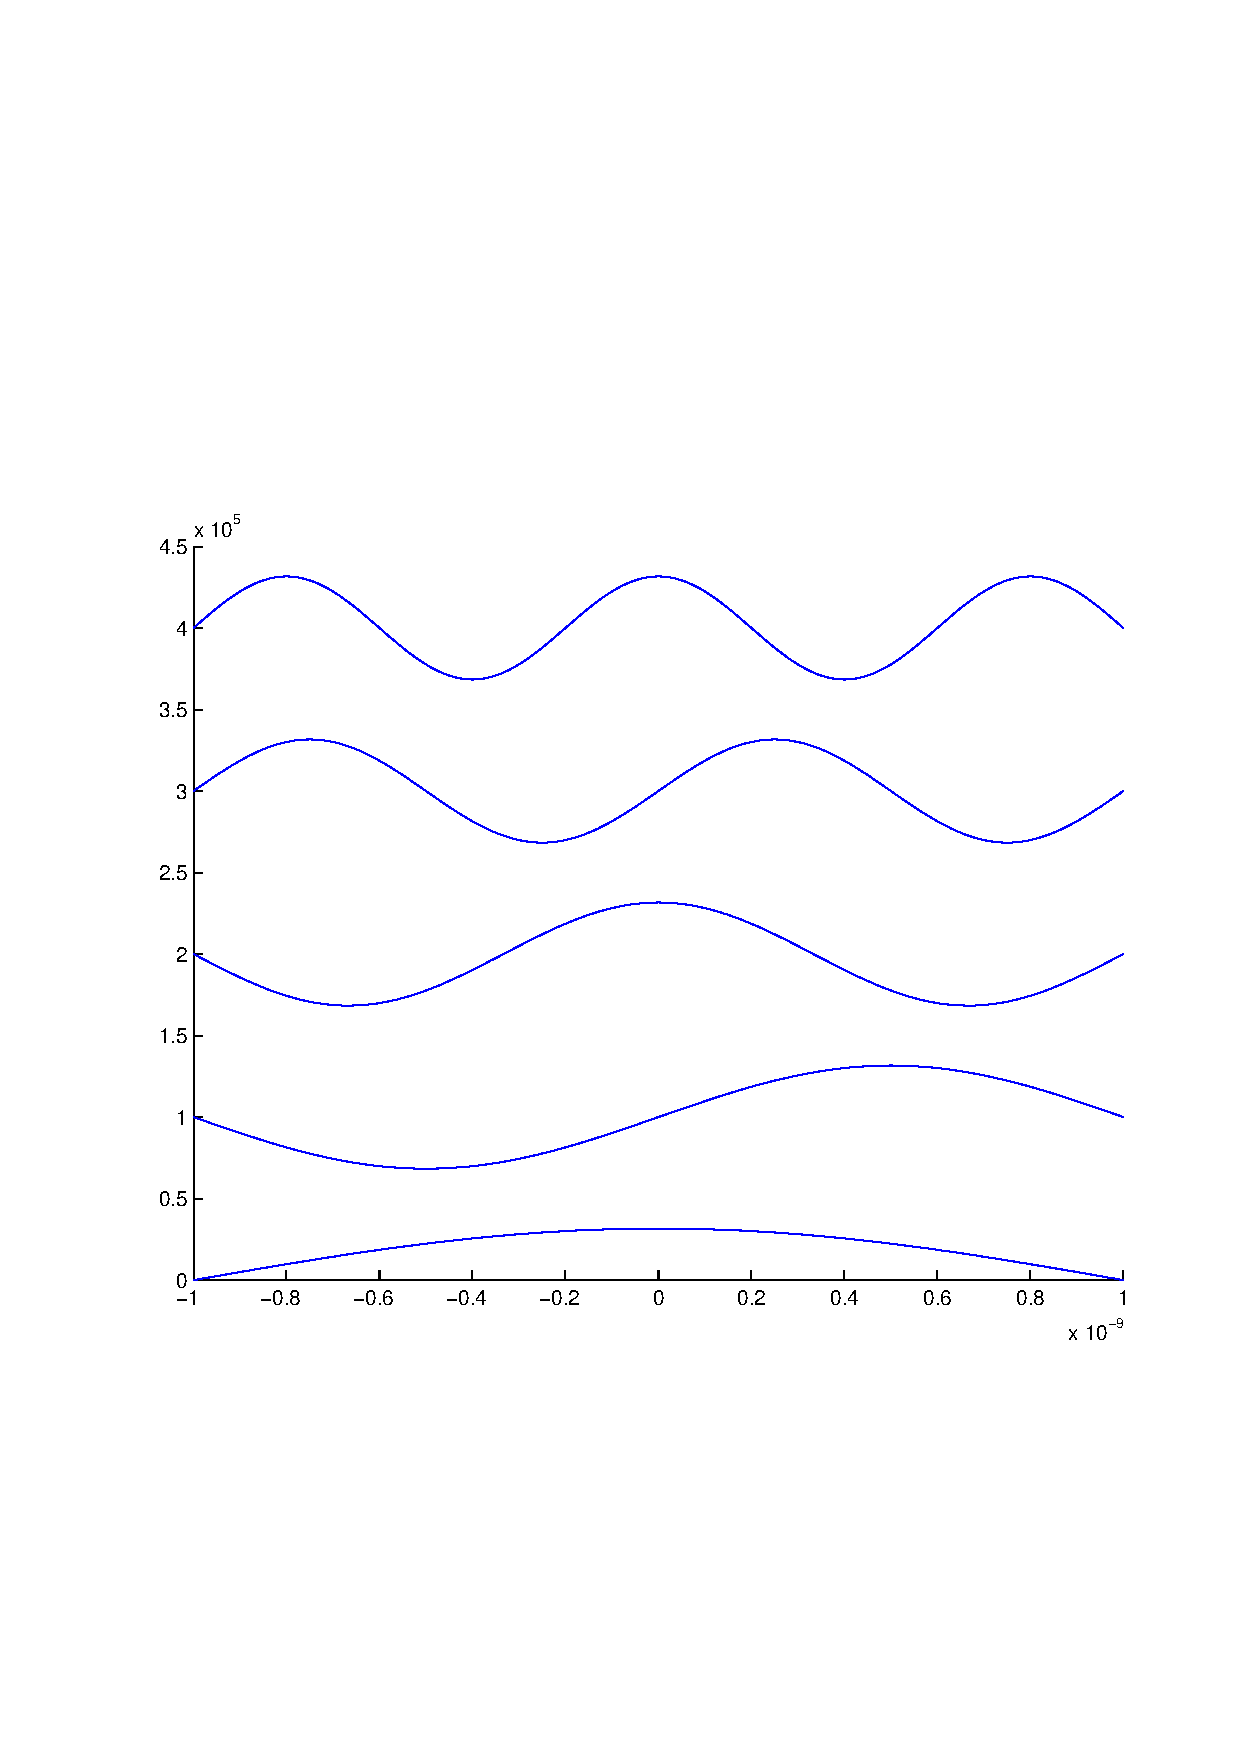
\includegraphics[width=12cm,clip=true,trim=2cm 7cm 1cm 8cm]{efeld/Psi_ungestoert.pdf}
 \caption{$\psi$ ungest\"ort}
 \label{abb:efeld_psi_ungestoert}
\end{figure}

Bei unserer Anwendung bauen wir auf dem Potentialkasten (Kapitel \ref{subsection:potentialkasten}, Seite \pageref{subsection:potentialkasten}).

Dabei geht es um ein Elektron welches zwischen zwei Barrieren mit unendlich hohem Potential gefangen ist.
Zwischen den Barrieren kann sich das Teilchen mit den Wellenfunktionen $\psi_k$ bewegen,
ausserhalb kommt es hingegen nicht vor.

Wir erweitern jetzt das System mit einer St"orung, indem wir eine elektrische Spannung anlegen.
Weil das Elektron eine negative Ladung besitzt ver"andert sich seine Wellenfunktion.

%fixme: negatives Elektron

Als Grundlage "ubernehmen wir zwei Funktionen aus dem Skript
\begin{equation}
\begin{aligned}
H^{(0)}&=\frac1{2m}p^2+V^{(0)}(x)
\\
V^{(0)}(x)&=
  \begin{cases}
    0       & \qquad |x|<l\\
    \infty  & \qquad\text{sonst}
  \end{cases}
\end{aligned}
\end{equation}

und erweitern sie mit der St"orung $V^{(1)}$, welche wir als lineares Feld definieren:
\begin{equation}
  V^{(1)}(x) = a x + b
\end{equation}

Die St"orung kann noch weiter vereinfacht werden:

Da wir $a$ bereits durch $\varepsilon$ beschreiben, k\"onnen wir mit $a = 1$ vereinfachen,
und weil die Barrieren unendlich hoch sind, k"onnen wir $b = 0$ setzen.

Wenn wir jetzt die St"orung einsetzen, bekommen wir die neue Hamilton-Funktion
\[
  H=\frac1{2m}p^2+V^{(0)}(x)
    + \varepsilon x.
\]
aus welcher wir den Hamilton-Operator berechnen k"onnen:
\[
  \hat{H} = -\frac{\hbar^2}{2m} \frac{\partial^2}{\partial x^2} + V^{(0)}(x) + \varepsilon x
\]

\subsubsection{Vorgehensweise}
Wir berechnen in unserem Beispiel die erste N"aherung.

Im Kapitel \ref{skript:stoerungsloesung1ordnung} wird beschrieben wie man von der Schr"odingergleichung 
auf die erste N"aherung kommt.

Entscheidend hier ist ob die Zust"ande entartet sind oder nicht.
Entartung bedeutet, dass zwei Zust"ande die selbe Energie besitzen, wodurch der Nenner zu Null wird.
Das w"are der Fall wenn das Elektron aus dem Kasten entkommen w"urde,
dann h"atten zwei Wellen ausserhalb des Kastens die selbe Energie.

Diesen Fall schliessen wir mit den unendlich hohen Barrieren aus.

Wir benutzen also folgende Funktionen
\begin{equation}
\begin{aligned}
E_k^{(1)} &=
\langle \psi_k^{(0)}|\, H_1 \,|\psi_k^{(0)}\rangle
\\
|\psi_k(\varepsilon)\rangle &=
(1+i\varepsilon \gamma)
\,|\psi_k^{(0)}\rangle
+
\varepsilon
\sum_{k\ne l}
\frac{\langle \psi_l^{(0)}|\, H_1 \,|\psi_k^{(0)}\rangle}{E_k^{(0)}-E_l^{(0)}}
\,
|\psi_l^{(0)}\rangle
\end{aligned}
\end{equation}

Mit der ersten Gleichung k"onnen wir direkt die Energie der St"orung berechnen.

Man berechnet das Skalarprodukt von $\psi_k^{(0)}$ und $x \psi_k^{(0)}$ "uber 
die gesamte L"ange des Potenzialkastens und erh"alt so die Energie der St"orung $E_k^{(1)}$.

Diese setzt man jetzt in $E_k(\varepsilon)=E_k^{(0)} + \varepsilon E_k^{(1)}$ ein und bekommt so die st"orungsabh"angige Energie.

Um $\psi_k(\varepsilon)$ zu berechnen wird es etwas schwieriger, weil sich in der Quantenmechanik die Energiezust"ande $k$ gegenseitig beeinflussen.

Wir setzen daher eine St"orung $\psi_k^{(1)}$ aus mehreren $\psi_k^{(0)}$ zusammen.
Mit der zweiten Formel k"onnen wir den Anteil der jeweiligen $\psi$ berechnen.

Wir berechnen also die Summe aller $\langle\psi_l^{(0)}|\psi_k^{(0)}\rangle|\psi_l^{(0)}\rangle$
und bekommen so $\psi_k^{(0)}$.
Die Welle $\psi_k^{(0)}$ hat hierbei keinen Anteil in der St"orung $\psi_k^{(1)}$,
denn $\langle \psi_k^{(0)}|\, H_1 \,|\psi_k^{(0)}\rangle$ ergibt ja die Energie der St"orung.







\begin{equation}
  \label{eq:efeld_skalar_gleichung}
  \langle\psi_l^{(0)}|\psi_k^{(1)}\rangle
      =
  \frac{\langle \psi_l^{(0)}|\, H_1 \,|\psi_k^{(0)}\rangle}{E_k^{(0)}-E_l^{(0)}}
\end{equation}

Die Formel \ref{eq:efeld_skalar_gleichung} ergibt einen Skalarwert, welchen Anteil die Welle $l$ an der St"orung $k$ hat.









\subsubsection{Berechnung des Modells mit Matlab}

Wir wollen jetzt die Wellen $\psi_k(\varepsilon)$ und die Energie auch tats"achlich berechnen.
Dazu verwenden wir das Programm Matlab.

Matlab (MATrix LABoratory) ist ein Programm welches sich gut zum Plotten von Funktionen
und zum Berechnen von Matrizen eignet.
Besonders das berechnen von Matrixen und Vektoren wird durch den Syntax der eigenen Programmiersprache erleichtert.

Hier ein paar Befehle welche zum Verst"andnis n"utzlich sind:
\begin{itemize}
\item Mit \\
\begin{lstlisting}vektor = n : m\end{lstlisting} \\
wird von $n$ bis $m$ gez"ahlt
\item Mit
%\begin{lstlisting}vektor = n : delta : m\end{lstlisting}
wird ein Vektor mit Werten von $n$ bis $m$ definiert die den Abstand delta haben.
\item Mit
%\begin{lstlisting}vector(:)\end{lstlisting}
k"onnen alle Werte aus einem Vektor ausgelesen werden.
\item
%\begin{lstlisting}vector*vector\end{lstlisting}
entspricht einem Skalarprodukt.
\item
%\begin{lstlisting}vector.*vector\end{lstlisting}
entspricht der Elementweisen Multiplikation.
\end{itemize}

Wie beginnen damit das wir Konstanten und das ungest"orte System bestimmen.

Wir definieren f"ur unseren Potenzialkasten eine Breite von $10^-9$ (1nm links und rechts)
\begin{lstlisting}[style=Matlab]
L = 10^-9;
xSteps = 250;
x = -L : 2*l/xSteps : +L;
\end{lstlisting}
und bekommen so den Vektor x.

Um die ungest"orten Zust"ande $\psi_k^{(0)}$ zu bekommen, k"onnen wir die Sinus- und Kosinus-Funktion diskret abtasten.

Wir berechnen ausserdem die Energien $E_k^{(0)}$

\begin{lstlisting}[style=Matlab]
m = 9.10938291*10^-31;		% Elektronenmasse
h = 6062606957*10^-34;		% Planck-Konstante

for k = 1 : 1000
    E(k) = h^2*k^2 / (32*m*L^2);
    
    if mod(k, 2) == 0
        y = sin(k*pi*x/(2*L));
    else
        y = cos(k*pi*x/(2*L));
    end
    Psi(ln, x) = 1/sqrt(2*L) .* y;
end
\end{lstlisting}

Wir bekommen so einen Vektor mit den Werten f"ur $E_k^{(0)}$
und eine Matrix 500 mal 1000 f"ur $\psi_k^{(0)}$.

Nun da wir die Grundlagen berechnet haben, k"onnen wir $\psi_k(\varepsilon)$ und $E_k(\varepsilon)$ berechnen.

Wir k"onnen die Energie mit
\begin{lstlisting}[style=Matlab]
...
H1 = x;
for k = 1 : 5
  E1(k) = dot(Psi(k, :), H1.*Psi(k, :));
  plot(epsilon, E0(k) + epsilon*E1_k(k))
end
\end{lstlisting}
berechnen und plotten, wobei dot(a, b) das Skalarprodukt bildet.

Das Resultat sehen wir in der Abbildung \ref{abb:efeld_E_gestoert}.

Die Implementierung von $\psi_k^{(0)}$ ist wegen $\sum$ etwas schwieriger.

Normaler Weise k"onnte man mit sum(vektor) alle Elemente zusammenz"ahlen.
Wir wollen aber ja ein Element auslassen.

Um zum Beispiel den f"unften Zustand $\psi_5^{(1)}$ zu bestimmen addieren wir alle 
$\langle\psi_l^{(0)}|\psi_5^{(1)}\rangle|\psi_l^{(0)}\rangle$
 von 1 bis n ausser 5.
\begin{equation}
  \sum_{l=1 ; l\ne 5}^{\infty}
    \frac{\langle \psi_l^{(0)}|\, H_1 \,|\psi_k^{(0)}\rangle}{E_k^{(0)}-E_l^{(0)}}
        \,
    |\psi_l^{(0)}\rangle
\end{equation}

In Matlab wird das wie folgt implementiert:
\begin{lstlisting}[style=Matlab]
H1 = x * -1;          # Die Stoerung des elektrische Feldes mit dem
                      #   Faktor -1, da das Elekton negativ geladen ist
n = 1000;             # Anzahl aufsummierte Zustaende
k = 5;                # Der Zustand den wir plotten
summe = 0;            # Initialisierung des SummenVektors

for l = 1 : n
  if l ~= k           # Vergleich l ungleich k
    Psi_lk = dot(Psi(l, :), H1.*Psi(k, :)) / (E(k)-E(l)) .* Psi(l, :);
    summe = summe + Psi_lk;
  end
end
\end{lstlisting}
$summe$ ist nun ein Vektor mit den diskreten Abtastwerten von $Psi_k^(1)$.

Beim Aufsummieren zahlt es sich aus nicht alle Zust\"ande zu ber\"ucksichtigen, weil der Anteil am Gesammtzustand 
mit jedem Schritt weiter abnimmt. Der Grund ist die stetige Zuname des Terms $E(k)-E(l)$ unter dem Bruchstrich.

In diesem Fall addieren wir beim 90-sten Schritt ($l=90$) nur $1\%$ der St"orung dazu.
Beim 280-sten Schritt ($l=280$) betr\"at der Anteil nur noch $0.1\%$.

Wir k"onnen jetzt die St"orung in 
\begin{equation}
|\psi_k(\varepsilon)\rangle
=
(1+i\varepsilon \gamma)
\,|\psi_k^{(0)}\rangle
+
\varepsilon|\psi_k^{(1)}\rangle
\end{equation}
einsetzen und bekommen so die neue Wellenfunktion in Abbildung \ref{abb:efeld_psi_gestoert}.


















\subsubsection{Auswertung Psi}

\begin{figure}
 \centering
 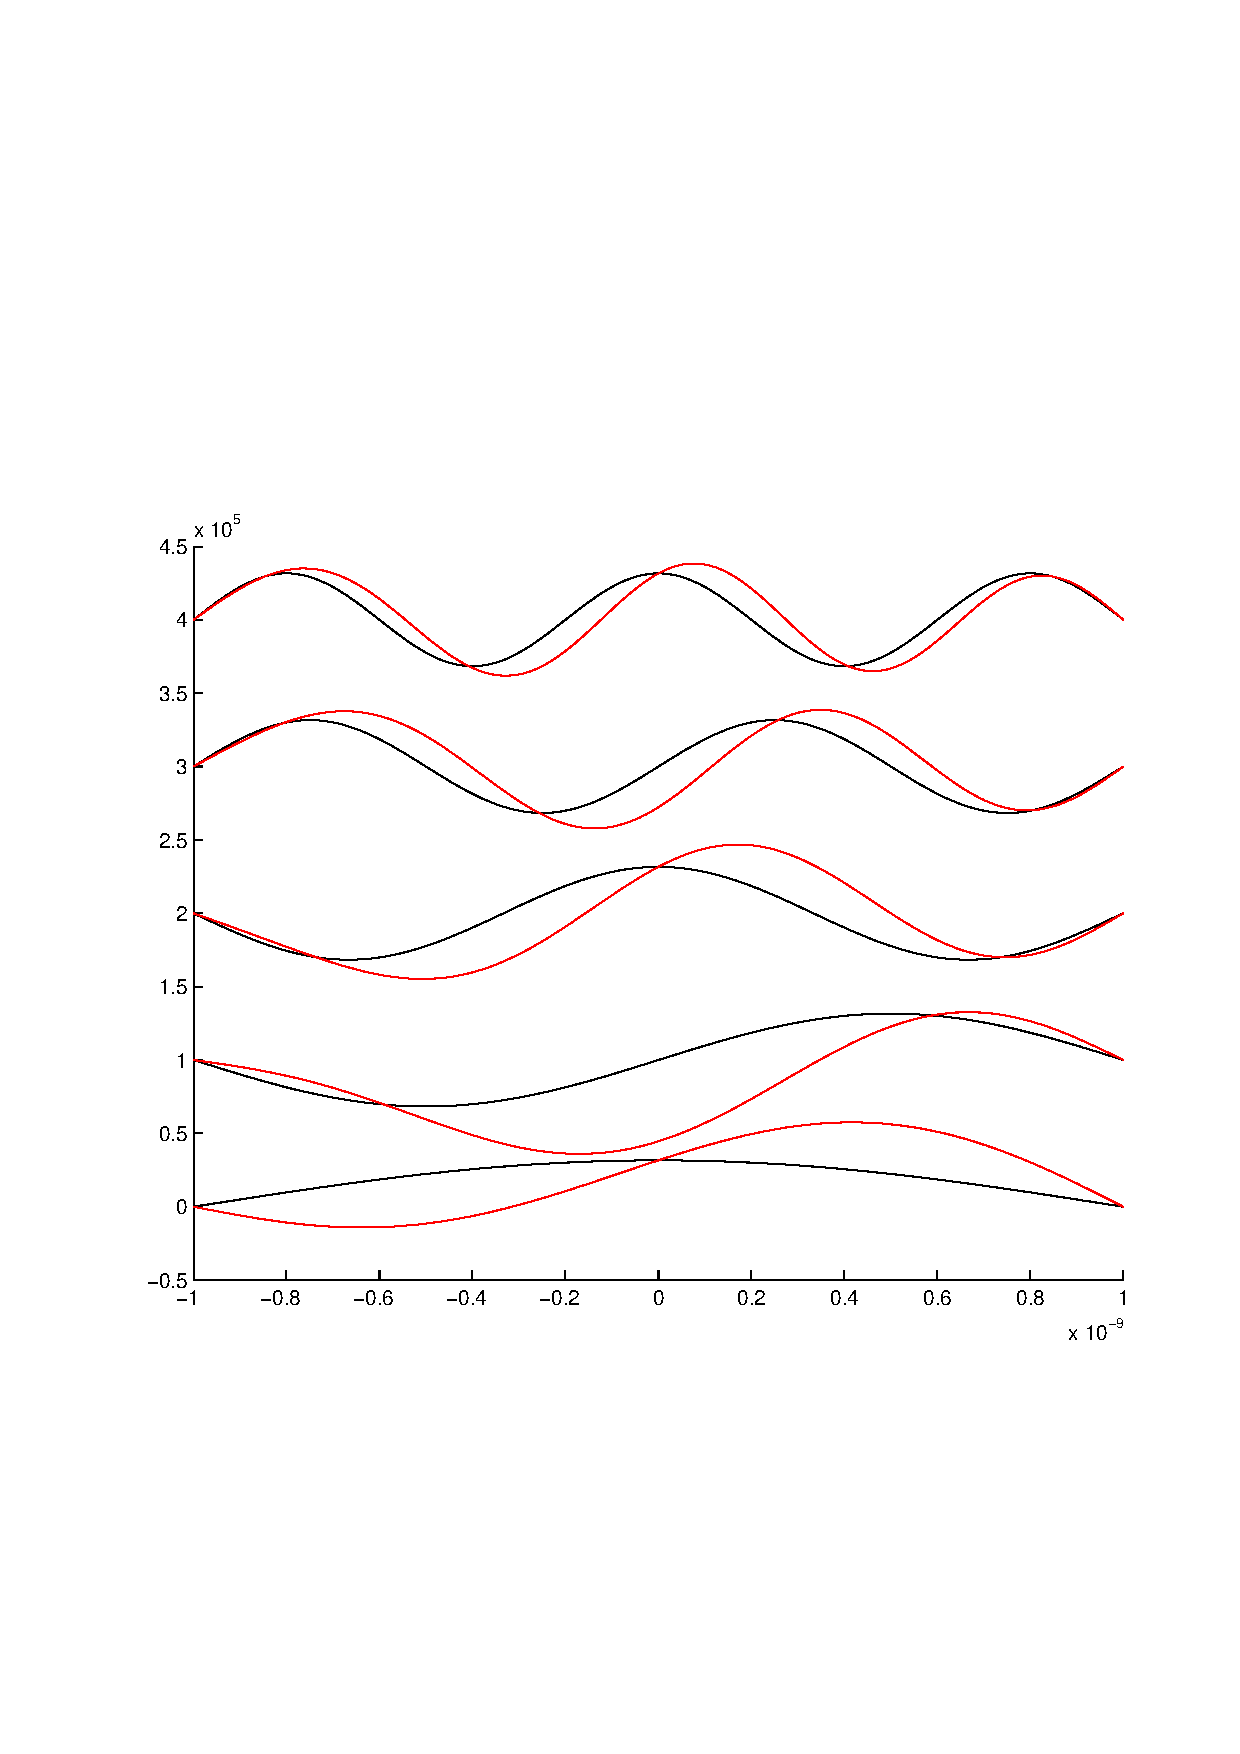
\includegraphics[width=12cm,clip=true,trim=2cm 7cm 1cm 8cm]{efeld/Psi_gestoert.pdf}
 \caption{$\psi$ gest\"ort}
 \label{abb:efeld_psi_gestoert}
\end{figure}

In der Grafik \ref{abb:efeld_psi_gestoert} sehen wir die Unterschiede zwischen dem normalen $\psi$ (schwarz) \& der ersten N"aherung (rot).

Auf der vertikalen Achse haben wir die Amplituden von $\psi_k$.
$\psi^2$ entspricht der Wahrscheinlichkeitsdichte das sich das Elektron an dieser Stelle befindet.

Auf der Horizontalen sehen wir die x-Position vom Teilchen im eindimensionalen Potentialkasten.

Intuitiv nimmt man an, dass die Wellenfunktion nach links gedr"uckt werden wird, da die monoton steigende St\"orung
des elektrischen Felds $x$ im ersten Quadranten ein positives Potential bildet.
% FIXME Satz korrekt?
Dieser Eindruck ist dem Fakt geschuldet, dass das Elektron den Berg aus Wiederstand herunterrollen m\"ochte.

Die Intuition ist tr\"ugerisch. Durch das positive Potential wird das Elektron angezogen \& die
Wahrscheinlichkeit es weiter Rechts bei einem h\"oheren $l$ anzutreffen steigt.

Die Energie des Elektrons wird durch die St\"orung verschoben.
Der Ausgleich wird in der Schr"odingergleichung beschrieben:
\[
-\frac{\hbar^2}{2m}\Delta\Psi(x) + V(x)\Psi(x)
=
E \Psi(x)
\]

% FIXME was
Weil $E \Psi(x)$ konstant ist, sinkt bei einem h"oherem Potential $-\frac{\hbar^2}{2m}\Delta\Psi(x)$,
was einer Abnahme der Frequenz entspricht.

Wir haben in dieser Abbildung das Epsilon sehr stark gew"ahlt,
weil bei einem schwachen Epsilon die "Anderungen nur schlecht sichtbar sind.



\subsubsection{Auswertung E}

In der Grafik \ref{abb:efeld_E_gestoert} lassen wir f"ur die jeweiligen stabilen Zust"ande 0..4 
den Einfluss der St"orung wachsen.

Da das elektrische Feld jedoch nur einen sehr kleinen Einfluss auf die gesamte Energie des 
Elektrons hat, mussten wir um die Effekte der 1. N"aherung zu zeigen ein sehr grosses $\varepsilon$
w"ahlen.

\begin{figure}
 \centering
 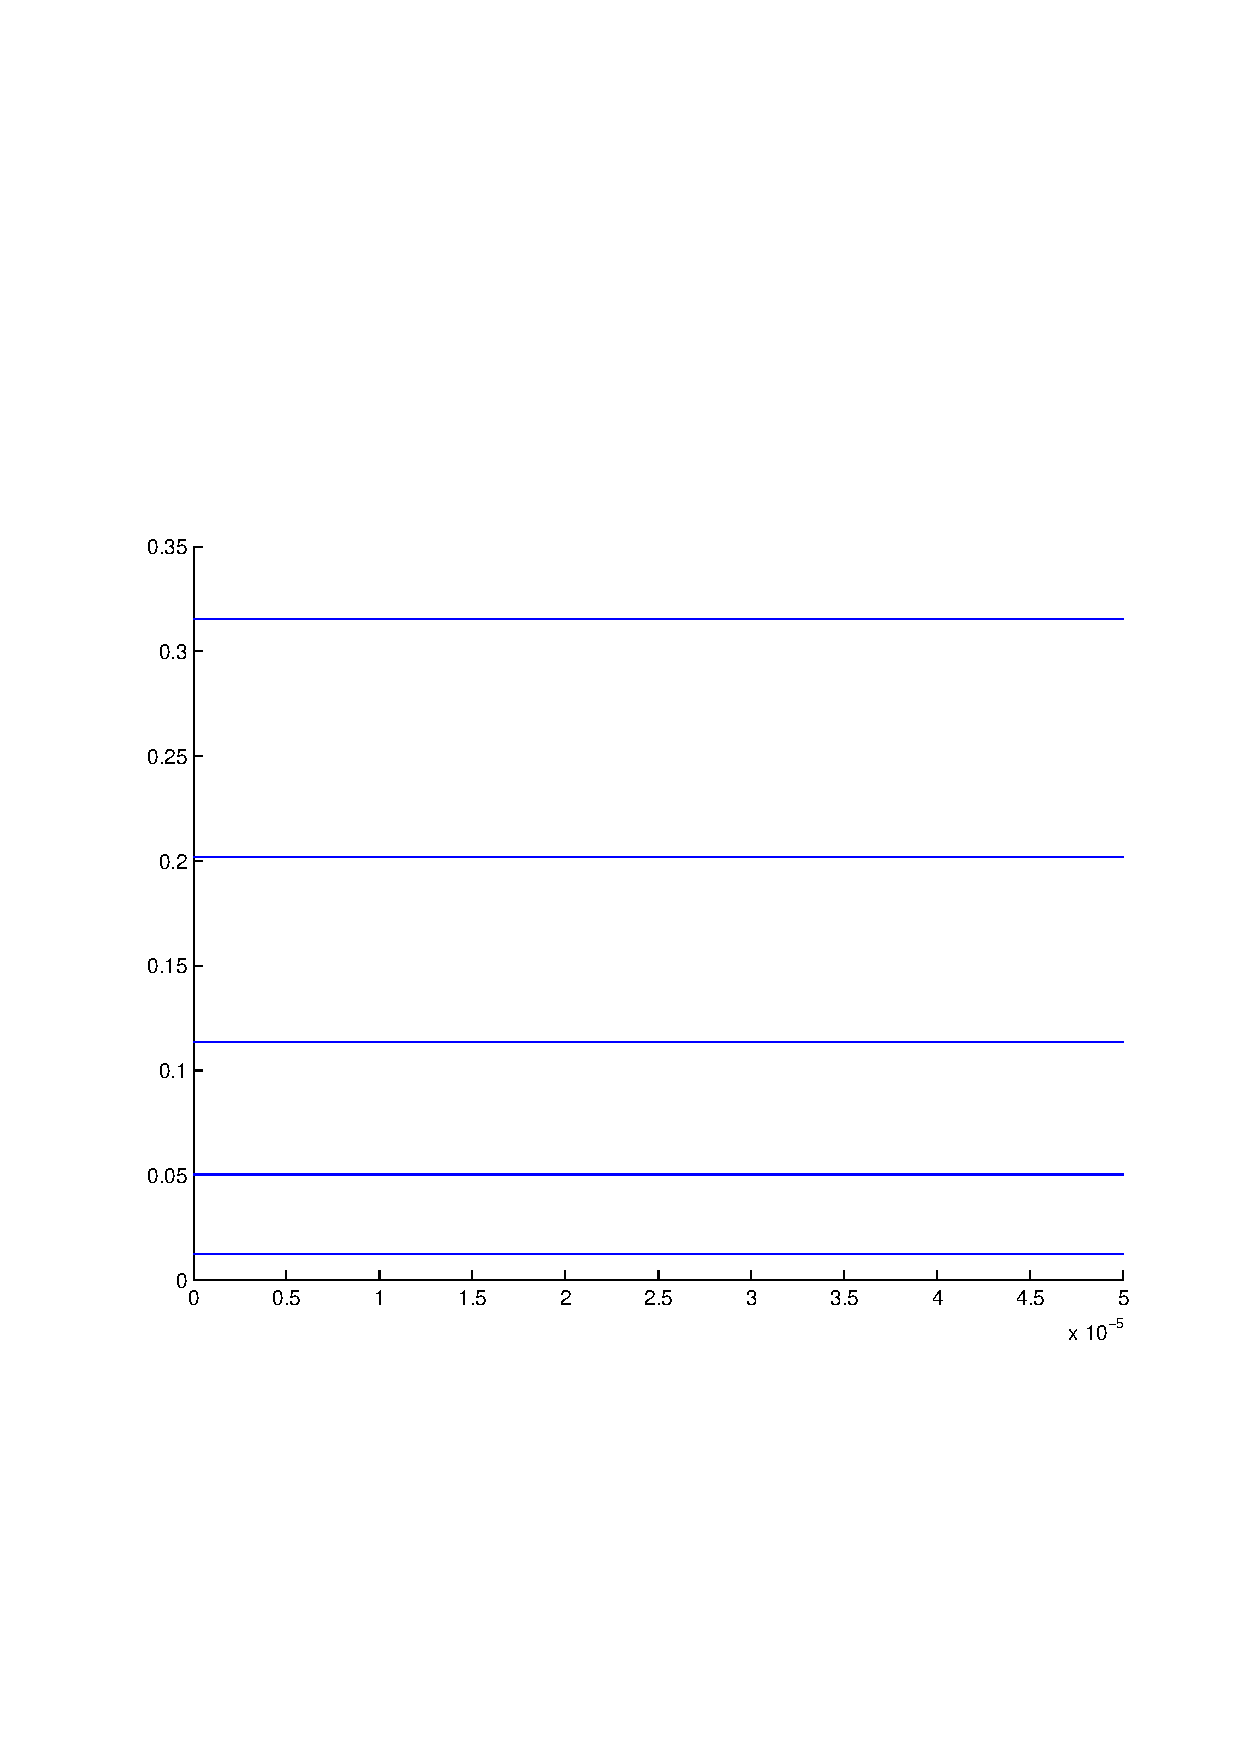
\includegraphics[width=12cm,clip=true,trim=2cm 7cm 1cm 8cm]{efeld/Energie_gestoert.pdf}
 \caption{$E$ gest\"ort, x-Achse ist $\varepsilon$, y-Achse ist die gesammte Energie des Systems}
 \label{abb:efeld_E_gestoert}
\end{figure}







\printbibliography[heading=subbibliography]
\end{refsection}
